%*******************************************************************************
%****************************** Second Chapter *********************************
%*******************************************************************************

\chapter{Learning Resource Database based on Knowledge Graph}

\ifpdf
    \graphicspath{{Chapter2/Figs/Raster/}{Chapter2/Figs/PDF/}{Chapter2/Figs/}}
\else
    \graphicspath{{Chapter2/Figs/Vector/}{Chapter2/Figs/}}
\fi


\section{Research Motivation}
As the starting point of a recommendation system, the data source is often the first step to consider.
在这里我们


A knowledge graph is a map that serves as a kind of knowledge domain mapping, which shows the knowledge development process and structure. Visualization techniques are used to describe knowledge resources and their carriers, to mine, analyze, construct, map and display knowledge and their interconnections. Also knowledge graphs, as an important part of artificial intelligence, are now playing an increasingly important role in recommendation systems and question and answer systems.

In this section, this paper uses the knowledge graph to store the knowledge points and questions of high school mathematics as the data source for the recommendation system. It serves as a supplementary input to the knowledge tracing model section and provides a priori knowledge of the subject knowledge points.

Firstly, the basic principles and common techniques of knowledge graph are introduced, and then a knowledge graph construction method for automatic extraction of knowledge points of test questions is proposed, and the knowledge graph construction and knowledge point extraction, corpus acquisition and preprocessing, knowledge point identification and knowledge graph updating techniques are introduced.

In this paper, we will use the knowledge graph in constructing the knowledge graph of mathematics domain and building the student user model. In the construction of the knowledge graph of high school mathematics domain, the basic concepts and keywords involved in the textbooks are abstracted into knowledge point ontologies, the knowledge point keywords in high school mathematics exercises are identified by the named entity recognition method, and then the abstracted knowledge points are associated with the keywords to build the knowledge graph of high school mathematics. A large number of knowledge points in high school mathematics are associated with the degree of mastery of each knowledge point by individual students, which is built into a student user model, and the abstraction of the student user model into a knowledge graph will facilitate the personalized recommendation of exercises.

\section{Research Status}


\section{Basic theory of knowledge graph}
The Knowledge Graph is a new concept introduced by Google in 2012. Knowledge graph is essentially a knowledge base of Semantic Network, which describes conceptual entities and their relationships in the objective world in a structured form. From the beginning of oogle search, to nowadays chatbots, big data risk control, securities investment, intelligent medical care, adaptive education, recommendation system, all use knowledge graph.

\subsection{Representation}
Knowledge graphs focus on concepts, entities and their relationships, where entities are things in the objective world and concepts are generalizations and abstractions of things with the same properties. Ontology is the basis of knowledge representation of knowledge graph, which can be formally represented as $O=\{C,H,P,A,I\}$, where $C$ is the set of concepts, such as transactional concepts and event-like concepts, $H$ is the set of contextual relations of concepts, $P$ is the set of attributes, which describes the features possessed by concepts, $A$ is the set of rules, which describes the domain rules, and $I$ is the set of instances, which describes the instance-attribute-value.

The common knowledge graph representations are Resource Description Framework (RDF), Resource Description Framework Schema (RDFS), Web Ontology Language (OWL), etc.

\begin{enumerate}
\item resource description framework RDF is the most commonly used symbolic semantic representation model, which provides a unified standard for describing entities/resources. the basic model of RDF is a directed labeled graph, each edge on the way corresponds to a subject-predicate object triad, and a triad corresponds to a statement of an event. the RDF consists of nodes and edges, the nodes represent entities/resources, attributes, and the edges represent entities and the relationship between entities and attributes. Figure \ref{triad1} shows the relationship between entities and attributes.
\item lightweight schema language RDFS is an extension of RDF by adding the definition of class properties and other Schema layers on top of the objective events provided by RDF. rdfs is mainly used to define term sets, class sets and property sets, mainly including classes, subclasses, properties, subclass properties, domains, scopes and other primitives, which can build the basic class hierarchy and These clauses can build the basic class hierarchy and attribute system.
\item OWL is the core of the Semantic Web technology stack, which provides fast and flexible data modeling capability and efficient automatic reasoning capability.
\end{enumerate}

\begin{figure}[h]
  \centering
  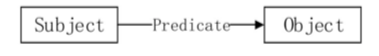
\includegraphics[width=0.8\textwidth]{f01}
  \caption{Structure of Triad}
  \label{triad1}
\end{figure}

\subsection{Storage}
There are mainly two kinds of storage for knowledge graphs, one is based on the academic idea of RDF, which is based on triples car storage: the other is based on the industrial idea of attribute graph, which is based on attribute graph storage.

Using RDF for storage, mainly RDF serialization methods, such as RDF/XML, N- Triples, Turtle, RDFa, JSON-LD, etc.

The most important feature of the graph database for storing knowledge graphs is that the graph database can store not only the nodes and relations of triples, but also the attributes of their nodes and relations together, and the graph can be traversed efficiently, which is convenient for publishing data and retrieval of knowledge graphs.

\section{The construction of knowledge graph}
In order to convert a large number of standard questions into feature questions in a timely manner, this paper proposes an automatic knowledge extraction method based on knowledge graph for test questions. The method uses natural language processing techniques such as named entity recognition, keyword extraction and calculation of semantic similarity of keywords to collect knowledge points and mathematics-related vocabulary in high school mathematics domain and build up a knowledge map of high school mathematics. The mathematics test questions are divided into words and entities by customized dictionaries and rules, and the candidate keywords are extracted and brought into the knowledge map of high school mathematics for querying.

\subsection{The extraction of knowledge point}
In this paper, the architecture for building the knowledge map of high school mathematics is mainly divided into four modules: corpus collection module, pre-processing module, knowledge map building module and knowledge extraction system module. The high school mathematics mapping consists of two entities: mathematical knowledge points and mathematical vocabulary related to mathematical knowledge points, which are mainly used to provide automatic knowledge extraction function for the construction of intelligent question bank later. The question bank not only contains a large number of mathematical knowledge points, but also contains a lot of mathematical vocabulary related to mathematical knowledge points. The mathematical vocabulary does not only stop at the mathematical concept ontology, mathematical textbook chapter names, mathematical knowledge points, etc., but also includes words or vocabulary that can deduce the knowledge points of the test questions. For example, if the operation symbol of "∩" appears in the question, it can be deduced that the question is probably about "set", "set operation", "set intersection operation", "set element interdependence", "set interval", "set interval", "set interval", "set interdependence", "set interval", etc. "The pre-processing module is to standardize the imported data corpus to form structured data, and then to identify the named entities, which mainly involves the process of entity identification and relationship extraction. High school mathematics is relatively a semi-closed and semi-open subject, the mathematical knowledge is relatively closed, but the mathematical test questions are very different, but the final solution still comes back to the test mathematical knowledge, so it is semi-open. The relevant mathematical knowledge points and concepts obtained through knowledge extraction need to be evaluated by experts to create a valuable and credible knowledge map. The knowledge extraction system plays a key role in the construction of the intelligent question bank by tagging the questions obtained by crawlers on the web after processing. 

\subsection{Corpus data preprocessing}
After importing the textbook and web crawler corpus, although a large amount of valuable text, image information and structured data such as question stems and parses in the question bank have been obtained, there are a large number of mathematical formulas in these data, and these mathematical formulas are not standardized because of the platform, and there is no uniform storage format, so it is necessary to standardize these text data containing mathematical formulas.



\begin{itemize}
	\item standardization: The standardization process is mainly for the pictures and mathematical formulas in the corpus, many crawlers get the test information through the pictures, the test information stored in the pictures is very unfavorable to the word separation and naming entity recognition, and the mathematical formulas also exist in a variety of storage methods, currently more common storage and display of mathematical formulas are Office comes with the formula editor plug-in, Mathtype formula editor, Mathml, Latex and so on. For picture information, we use OCR technology for text recognition, and for mathematical formulas, we use Latex format. Mathpix is a software for quickly recognizing mathematical formulas stored in pictures and converting them into Latex format with high recognition accuracy and efficiency, and Latex can extract some useful semantic information for later knowledge extraction when expressing mathematical formulas.
	\item User dictionaries and stopwords: User dictionaries, also known as user-defined dictionaries, are mainly used to enhance the disambiguation and error correction ability of the subscripts by manually adding subscripts rules in the process of named entity recognition, and the subscripts recognition will give priority to the words in the user dictionaries for subscripts after adding the user dictionaries. At present, there is no mature lexical corpus in the field of mathematics, so it is important to build a user lexicon related to mathematics. For example, if we do not add a user lexicon for "function analytic", we will get [function, analytic, equation] if we use the popular third-party corpus Jieba, but we do not want to see such a result when we add the field "analytic" to the user lexicon. When the "parser" field is added to the user's dictionary, the result will be [function,parser]. Deactivated words are also called "dummy words in computer search, non-search words". In search engines, in order to save space and search efficiency, certain words or phrases are usually automatically ignored in search requests, and these words or phrases are called deactivated words. The deactivation dictionary is a filter composed of a number of deactivation words, in the named entity recognition of the word, the system can be based on the deactivation dictionary to filter out some of the words or words that are not useful, to improve the accuracy of the word and the system computing efficiency. Deactivated words mainly include common pronouns, inflectional auxiliaries, adverbs, prepositions, conjunctions, etc., which usually have no obvious meaning of their own and only have a certain role when they are put into a complete sentence, such as: [you, I, he, this, that, the, in, then], etc.
	\item Tokenization: In the process of constructing mathematical knowledge graphs, word separation is mainly used to obtain mathematical knowledge points and related mathematical vocabulary, so there is no strict requirement on the lexicality of the words obtained by word separation. In this paper, we use Hanlp natural language processing toolkit to classify the text by perceptual machine. Hanlp has the features of perfect function, high performance, clear architecture, new corpus and customizable. and can recognize new words
\end{itemize}

\section{Experiment}

\subsection{Dataset and Environment}

The accuracy of the knowledge point extraction directly affects the construction of the feature database. The experiment selected 100,000 and 500 high school mathematics test questions with knowledge points in the web crawler as samples, and divided them into two parts for the automatic extraction of knowledge points without and with expert audit. As shown in Table , the accuracy of knowledge point extraction is 72.3\% when there is no expert review and 96.6\% when there is expert review. This experiment shows that the real-time updating of the knowledge map of high school mathematics in the process of automatic knowledge point extraction is the key to improve the accuracy of knowledge point extraction.

\begin{table}[h]
	\centering

	\begin{tabular}{|l|l|l|}
	\hline
				& Without expert review & With expert review \\ \hline
	Sample Size & 100000                & 500                \\ \hline
	Accuracy    & 72.3\%                & 96.6\%             \\ \hline
	\end{tabular}
	\caption{The accuracy comparison table}
\end{table}

\subsection{Performance Indicators}


\subsection{Design of Experiment}

\subsection{Experiment Review}


\subsection{The Exercise Embedding }

\section{Summary}
This chapter introduces the automatic knowledge extraction method of test questions based on knowledge graph. The intelligent algorithm based on individual features proposes to convert the standard question bank into a feature bank with knowledge feature representation, and defines each dimension in the feature bank, constructs the individual feature bank for users according to individual knowledge points, and explains the recommendation algorithm of test questions in the intelligent question bank; the automatic extraction method of knowledge points of test questions based on knowledge map introduces the whole process of knowledge map of high school mathematics from corpus collection, construction, storage and update. This chapter also introduces the automatic extraction process of knowledge points of high school mathematics test questions. This chapter also presents a comparative experiment on the objectivity of feature database construction and the effectiveness of automatic knowledge point extraction, and the related analysis of the experimental results.